\chapter{Polarization of radiation}
\section{The wave equations}
We start with Maxwell's equations for vacuum \citep{RadiationProcesses}:
\begin{equation}
    \begin{aligned}
        \nabla \vctr{E} & = 0,\\
        \nabla \vctr{B} & = 0,\\
        \nabla \times \vctr{E} & = - \frac{1}{c} \frac{\partial \vctr{B}}{\partial t}, \\
        \nabla \times  \vctr{B} & = \frac{1}{c} \frac{\partial \vctr{E}}{\partial t},
    \end{aligned}
\end{equation}
where $\vctr{E}$ and $\vctr{B}$ are electric and magnetic fields, respectively, and no free charges or currents are present.
The system can be reduced to a simple vectorized wave equation:
\begin{equation}
    \begin{aligned}
        \square \vctr{E} = 0,\\
        \square \vctr{B} = 0,
    \end{aligned}
\end{equation}
where $\square = \frac{1}{c^2}\frac{\partial}{\partial t} - \Delta$ is D'Alembert operator.
Owing to the symmetrical form of Maxwell's equations, the solutions take the form of: 
%\red{why do you use square brackets, if there are no other brackets? first brackets are usually round }
\begin{equation}
    \begin{aligned}
        \label{eq:wave_sol}
        \vctr{E} = \vctr{r}_0^EE_0\exp\left(\vctr{k} \mul \vctr{r} - i \omega t\right), \\
        \vctr{B} = \vctr{r}_0^BB_0\exp\left(\vctr{k} \mul \vctr{r} - i \omega t\right),
    \end{aligned}
\end{equation}
where $E_0$ and $B_0$ are complex amplitudes, $\vctr{r}_0^E$ and $\vctr{r}_0^B$ are unit vectors, $\vctr{k}$ is the wave vector and $\omega$ is frequency \citep{RadiationProcesses}. 
Substitution of these solutions into Maxwell's equations reveals that $\vctr{k}$ is orthogonal to both $\vctr{r}_0^E$ and $\vctr{r}_0^B$, and that $\vctr{r}_0^E$ and $\vctr{r}_0^B$ are also orthogonal to each other.
Thus, if $\vctr{k} = k\vctr{n}$, where $\vctr{n}$ is unit vector, then $\vctr{n}$, $\vctr{r}_0^E$, and $\vctr{r}_0^B$ form an orthogonal basis.
As a result, the solution describes a transversal wave propagating in the $\vctr{n}$ direction, with $\vctr{E}$ and $\vctr{B}$ perpendicular to each other.
The last two Maxwell's equations also show that $E_0 = B_0$, and $\omega = ck$.

This solution possesses a number of features.
First of all, the vectors of electric and magnetic fields are orthogonal at any given moment, thus it is enough to consider properties of only one component, e.g., of electric field.
Secondly, the exponential factor in Eq.~\ref{eq:wave_sol} indicates that the fields vary sinusoidally in time.
Finally, the energy flux carried by the wave
%is determined by the factor $E_0$.
comes from the Poynting theorem \citep{RadiationProcesses}:
%\begin{equation}
%    U = \frac{1}{8\pi}\left(|\vctr{E}| ^ 2 + |\vctr{B}| ^ 2\right).
%\end{equation}
%This can be time-averaged to:
\begin{equation}
    \label{eq:poynting}
%    <U> 
\langle S \rangle = \frac{c}{8\pi}\left(\frac{1}{2}\mrm{Re}\left(E_0E_0^* + B_0B_0^*\right)\right) = \frac{c}{8\pi}|E_0|^2.
\end{equation}

\section{Polarization geometry}
\begin{figure}
    \resizebox{\linewidth}{!} {
        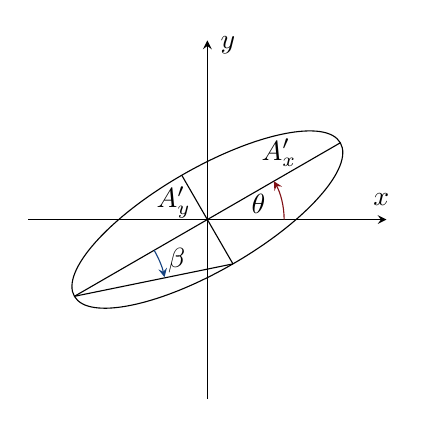
\begin{tikzpicture}[scale = 1.3, > = stealth]
            \draw[->] (-1.75, 0) -- (1.75, 0);
            \draw[->] (0, -1.75) -- (0, 1.75);
            \draw[rotate = 30] (0, 0) ellipse (1.5 and 0.5);
            \draw[rotate = 30] (-1.5, 0) -- (1.5, 0);
            \draw[rotate = 30] (0, -0.5) -- (0, 0.5);
            \draw[rotate = 30] (-1.5, 0) -- (0, -0.5);

            \draw[color={rgb,255:red,128; green,16; blue,21},-{>}] (0.75, 0) arc (0:30:0.75);
            \draw[color={rgb,255:red,21; green,66; blue,128}, rotate = 30, ->] (-0.6, 0) arc (0:-18:0.9);

            \draw (0.5, 0.15) node {$\theta$};
            \draw (-0.3, -0.4) node {$\beta$};
            \draw (0.7, 0.65) node {$A^\prime_x$};
            \draw (-0.33, 0.17) node {$A^\prime_y$};


            \draw (1.7, 0.2) node {$x$};
            \draw (0.2, 1.7) node {$y$};

        \end{tikzpicture}
    }
    \caption{
        Polarization ellipse. 
        $\theta$ determines \gls{PA}, $\beta$ -- ellipticity (and fraction of circular polarization).
        The semi-axes of polarization ellipse are determined by the amplitude of oscillation of electric vector and ellipticity: $A^\prime_x = |E_0|\cos \beta$, $A^\prime_y = |E_0| \sin \beta$.
        }
    \label{fig:ellipse}
\end{figure}
Eq.~\ref{eq:wave_sol} represents a monochromatic wave with a fixed direction of electric field (determined by $\vctr{r}_0^E$).
The behaviour of electric field as a function of time can be studied at some fixed $r$ using the following relationship: 
\begin{equation}
    \vctr{r}_0^EE_0\exp\left(\vctr{k} \mul \vctr{r} - i \omega t\right) = \vctr{r}_0^EE_0^\prime\exp\left(-i \omega t\right).
\end{equation}
In a coordinate system, where unit vector $\vctr{z}$ is collinear with $\vctr{k}$, and $\vctr{x}$, $\vctr{y}$ and $\vctr{z}$ form a right-handed coordinate system, vector $\vctr{E}$ oscillates in $xy$-plane.
It can be written as follows in a generalized scenario \citep{RadiationProcesses}:
\begin{equation}
    \label{eq:pol_proj_1}
    \vctr{E}(t) =  
    \begin{bmatrix}
        E_0^x \\
        E_0^y \\
        0
    \end{bmatrix} \exp\left(-i\omega t\right),
\end{equation}
where $E_0^x$ and $E_0^y$ are projections of complex $E_0$ onto $\vctr{x}$ and $\vctr{y}$, respectively.
Rewriting $E_0^x$ as $A_x\exp\left(i\phi_x\right)$ and $E_0^y$ as $A_y\exp\left(i\phi_y\right)$, $A_x$ and $A_y$ are real magnitudes, Eq.~\ref{eq:pol_proj_1} transforms into
\begin{equation}
    \label{eq:pol_proj_2}
    \vctr{E}(t) = 
    \begin{bmatrix}
        A_x\exp\left(i(\phi_x - \omega t)\right)    \\
        A_y\exp\left(i(\phi_y - \omega t)\right)    \\
        0
    \end{bmatrix}.
\end{equation}

The real part of Eq.~\ref{eq:pol_proj_2} describes how $\vctr{E}$ varies with time in a given point in space.
Switching to two-dimensional space of $xy$-plane, real part of $\vctr{E}$ has the following components:
\begin{equation}
    \label{eq:pol_proj_3}
    \mrm{Re} \vctr{E}(t) = 
    \begin{bmatrix}
    A_x \cos(\phi_x - \omega t) \\
    A_y \cos(\phi_y - \omega t) 
    \end{bmatrix}.
\end{equation}
Thus, the trajectory the electric field vector draws within $xy$-plane is an \textit{ellipse}.
The shape and orientation of said ellipse is determined by $A_x$, $A_y$, $\Delta\phi = \phi_x - \phi_y$.
The geometrical property of oscillation of electric field vector defines the polarization of the monochromatic wave.


Fig.~\ref{fig:ellipse} shows the schematic representation of the polarization ellipse.
From Eq.~\ref{eq:pol_proj_3} it follows that 
\begin{equation}
    \begin{aligned}
        \frac{E_x}{A_x} & = \cos\phi_x \cos (\omega t) + \sin \phi_x \sin(\omega t), \\
        \frac{E_y}{A_y} & = \cos\phi_y \cos (\omega t) + \sin \phi_y \sin(\omega t).
    \end{aligned}
\end{equation}
Eliminating $\omega t$, the system transforms into a general ellipse equation \citep{PolarizedLight2}:
\begin{equation}
    \label{eq:ellipse_1}
    \left(\frac{E_x}{A_x}\right)^2 + \left(\frac{E_y}{A_y}\right)^2 - 2\frac{E_x E_y}{A_x A_y}\cos(\Delta \phi) = \sin^2 (\Delta \phi).
\end{equation}
One of the main parameters of polarization ellipse is its position angle $\theta$.
Its value can be derived using the following approach.
If current two-dimensional coordinate system, determined by $\vctr{x}$ and $\vctr{y}$ unit vectors, is rotated by $\theta$, then ellipse equation is simplified to its standard form
\begin{equation}
    \label{eq:ellipse_2}
    \left(\frac{E_x^\prime}{A_x^\prime}\right)^2 + \left(\frac{E_y^\prime}{A_y^\prime}\right)^2 = 1,
\end{equation}
where $A_x^\prime$ and $A_y^\prime$ are unknown, and 
\begin{equation}
    \label{eq:ellipse_coord_rot}
    \begin{bmatrix}
        E_x^\prime\\
        E_y^\prime
    \end{bmatrix} =
    \begin{bmatrix}
        \cos \theta & \sin \theta \\
        -\sin \theta & \cos \theta
    \end{bmatrix}
    \begin{bmatrix}
        E_x \\
        E_y
    \end{bmatrix}.
\end{equation}
Substituting Eq.~\ref{eq:ellipse_coord_rot} into Eq.~\ref{eq:ellipse_2} and equating result to the r.h.s. of Eq.~\ref{eq:ellipse_1}, we arrive at \citep{PolarizedLight2}
\begin{equation}
    \theta = \frac{1}{2}\arctan\frac{2A_x A_y \cos (\Delta \phi)}{A_x^2 - A_y^2}.
\end{equation}

Angle $\beta$ (see Fig.~\ref{fig:ellipse}) determines the ellipticity of the trajectory.
It can be related to $A_y^\prime$ and $A_x^\prime$ as 
\begin{equation}
    \tan\beta = \frac{A_y^\prime}{A_x^\prime},
\end{equation}
as $A_x^\prime$ and $A_y^\prime$ are ellipse's semi-axes.
At the same time 
%\red{square root is missing in the denominators of the first two equations} 
\begin{equation}
    \begin{aligned}
        \label{eq:ellipt_angle}
        \sin \beta & = \frac{A_y^\prime}{\sqrt{{A_x^\prime}^2 + {A_y^\prime}^2}}, \\
        \cos \beta & = \frac{A_x^\prime}{\sqrt{{A_x^\prime}^2 + {A_y^\prime}^2}}, \\
        \sin (2\beta) & =  \frac{2 A_x^\prime A_y^\prime}{{A_x^\prime}^2 + {A_y^\prime}^2}.
    \end{aligned}
\end{equation}
From Eqs.~\ref{eq:ellipse_1}, \ref{eq:ellipse_2}
\begin{equation}
    \sin(2\beta) = \frac{2 A_x A_y}{A_x^2 + A_y^2} \cos (\Delta \phi).
\end{equation}

\section{Measuring polarization, Stokes parameters}
The polarization ellipse represents a trajectory, along which the tip of the vector of electric field  moves at a given point in space.
The characteristic time-scale of one revolution is $2\pi / \omega = 1/\nu$, where $\nu$ is frequency, which reaches $\sim 10^{14}$~Hz for visible light.
At the same time, the rate at which polarization is measured, is several orders of magnitude smaller. 
For instance, one polarimetric measurement per millisecond is only $1 / 10^{-3}~\mrm{s}^{-1} = 10^3$~Hz.
As a result, any observation of polarization of visible light records many trillions of oscillations of electric field, superimposed onto each other.
To estimate the observed properties of polarized light, Eq.~\ref{eq:ellipse_1} should be averaged over time, which reduces to an average over one period due to the nature of the electric field oscillations \citep{PolarizedLight2}:
\begin{equation}
    \label{eq:ellipse_avg}
    \frac{\langle E_x^2 \rangle }{A_x^2} + \frac{\langle E_y^2 \rangle }{A_y^2} - 2\frac{\langle E_x E_y \rangle }{A_x A_y}\cos(\Delta \phi) = \sin^2 (\Delta \phi),
\end{equation}
where, assuming period $T = 2\pi/\omega$,
\begin{equation}
    \langle f(t) \rangle  = \frac{1}{T}\int\limits_0^\mrm{T} f(t) \mrm{d}t.
\end{equation}
Owing to the sinusoidal nature of $E_x$ and $E_y$ variability in time,
\begin{equation}
    \begin{aligned}
        \langle E_x^2 \rangle    & = \frac{1}{2}A_x^2, \\
        \langle E_y^2 \rangle    & = \frac{1}{2}A_y^2, \\
        \langle E_x E_y \rangle  & = \frac{1}{2}A_xA_y\cos(\Delta \phi).
    \end{aligned}
\end{equation}
Eq.~\ref{eq:ellipse_avg} transforms into \citep{PolarizedLight2}
\begin{equation}
    (A_x^2 + A_y^2) ^ 2 - (A_x^2 - A_y^2) ^ 2 = (2 A_x A_y \cos(\Delta\phi)) ^ 2 + (2 A_x A_y \sin(\Delta \phi)) ^ 2.
\end{equation}
This equation can be rewritten in a vector form, introducing four new parameters:
\begin{align}
    \label{eq:stokes_abs}
    \begin{bmatrix}
        I\\Q\\U\\V
    \end{bmatrix} & = K
    \begin{bmatrix}
        A_x ^ 2 + A_y ^ 2 \\
        A_x ^ 2 - A_y ^ 2 \\
        2 A_x A_y \cos(\Delta \phi)\\
        2 A_x A_y \sin(\Delta \phi)
    \end{bmatrix},\\
    I^2 & = Q^2 + U^2 + V^2.
\end{align}
Here $I$, $Q$, $U$, and $V$ are absolute Stokes parameters of a fully polarized light \citep{Stokes1851}.
    $I$ is proportional to the total energy transmitted by the wave in a unit time.
    The scaling factor can be chosen so that $I$ Stokes parameter is equal to the energy flux $F$ (in units of energy per unit time and area), sometimes referred to as intensity \citep{PolarizationInCosmicMedium}.
    In this case, the scaling factor $K$ is $c/(16\pi)$ (from Eq.~\ref{eq:poynting}). 

In a general scenario, for partially polarized light the following inequality holds:
\begin{equation}
    I ^ 2 \ge Q^2 + U^2 + V^2,
\end{equation}
where $I$ is the total intensity, $I_\mrm{p} = \sqrt{Q^2 + U^2 + V^2}$ is the intensity of the elliptically polarized fraction \citep{Stokes1851}.
The parametric equations for the ellipse, expressed in two different coordinate systems, provide a way to write Stokes parameters in terms of geometrical parameters of the ellipse \citep{RadiationProcesses}:
\begin{equation}
    \begin{bmatrix}
        A_x \cos(\phi_x - \omega t) \\
        A_y \cos(\phi_y - \omega t)
    \end{bmatrix} =
    \begin{bmatrix}
        A_x^\prime \cos (\omega t) \\
        - A_y^\prime \sin (\omega t)
    \end{bmatrix}.
\end{equation}
Using Eq.~\ref{eq:ellipt_angle} and applying a rotation in a manner, similar to Eq.~\ref{eq:ellipse_coord_rot}, the equation transform into
\begin{equation}
    \label{eq:coord_connection}
    \begin{bmatrix}
        A_x \cos(\phi_x - \omega t) \\
        A_y \cos(\phi_y - \omega t)
    \end{bmatrix} = A
    \begin{bmatrix}
        \cos\beta\cos(\omega t)\cos\theta + \sin \beta \sin (\omega t) \sin\theta \\
        \cos\beta\cos(\omega t)\sin\theta - \sin\beta\sin(\omega t)\cos\theta
    \end{bmatrix},
\end{equation}
where $A^2 = A_x^2 + A_y^2$.
Evaluating Eq.~\ref{eq:coord_connection} at $\omega t = 0$ and $\omega t = \pi / 2$ yields
\begin{equation}
    \begin{aligned}
    A_x \cos\phi_x & = A \cos\beta\cos\theta, \\
    A_x \sin\phi_x & = A \sin\beta\sin\theta, \\
    A_y \cos\phi_y & = A \cos\beta\sin\theta, \\
    A_y \sin\phi_y & = -A \sin\beta\cos\theta.
    \end{aligned}
\end{equation}
Thus, Stokes parameters of the fully polarized light can be expressed as follows: 
% \red{should be $\sin$ in the last equation}
\begin{equation}
    \begin{bmatrix}
        I\\Q\\U\\V
    \end{bmatrix} = A^2
    \begin{bmatrix}
        1 \\
        \cos(2\beta)\cos(2\theta) \\
        \cos(2\beta)\sin(2\theta) \\
        \sin(2\beta)
    \end{bmatrix}.
\end{equation}
With such choice of angles, positive values of $\beta$ correspond to clockwise rotation of the electric field vector, while negative - to the counter-clockwise.

The form of the Stokes parameters reveals one of the most important properties of polarized light -- Stokes parameters of radiation, produced by several independent sources, can be added together, producing Stokes parameters that describe the combined beam.
Alternatively, this can be treated as the ability to decompose Stokes parameters of an arbitrary polarized light into basic components, namely unpolarized component (if present), linearly polarized (in different directions) and circularly polarized components.

\section{Broad-band polarization in astrophysics}
The emergence of polarization of radiation is usually associated with the existence of an asymmetry in the medium or in the emitting zone, or with a presence of a strong magnetic field.
There are physical processes that produce intrinsically polarized radiation \citep{RadiationProcesses}.
For instance, a charged particle moving in an ordered magnetic field produces magneto-bremsstrahlung, radiation caused by the particle acceleration, which includes cyclotron and synchrotron radiation.
Another example is polarization (and splitting) of spectral lines caused by the Zeeman effect \citep{PolarizationLines}.

Spectropolarimetric observations provide an important tool for studying magnetic fields in both degenerate \citep[e.g.,][]{Schmidt1995} and non-degenerate \citep{Mathys1989, Donati2009} stars.
Spectropolarimetry played an important role in developing the unified model of \glspl{AGN}.

Broad-band polarization usually reflects the geometrical properties of the source.
Supernovae exhibit broad-band polarization and polarized line features, which evolve over time \citep{Wang2008}.
Core-collapse supernovae tend to have relatively large broad-band polarization, which is likely caused by the asymmetry of explosions, while thermonuclear supernovae display very low continuum polarization, but a much larger line polarization, especially before the maximum light peak.
Peculiar stars such as Be \citep{Poeckert1979}, \gls{AGB} and post-\gls{AGB} \citep{Bieging2006} exhibit spectropolarimetric features as well.


Accreting compact objects are great examples of non-spherical emitters, therefore they may to produce polarized radiation.
Neutron stars are expected to polarize their X-ray radiation \citep[see, e.g., ][ for estimates]{Viironen2004, Loktev2020}, while stellar mass black holes demonstrate small optical polarization (e.g., \citealt{Russell2016}; \paperII; \paperIV; \inprepmaxi).

Finally, polarization also arises within the Solar system, where small Solar system objects reprocess light emitted by the Sun, introducing some degree of variable with phase angle linear polarization \citep[e.g.,][]{GoidetDevel1995, Penttila2005, Belskaya2019}.

The present work, however, focuses on the broad-band optical polarization.

\subsection{Emission from charged particles moving in magnetic field}
In the non-relativistic case, an electron gyrating around magnetic field line, produces radiation of the following polarization \citep{Ginzburg1964}: 
\begin{equation}
    \vctr{S}_\mrm{cycl} = \frac{\pi}{2} \omega_\mrm{B} \frac{v^2 e^2}{c^3} 
    \begin{bmatrix}
    1 + \cos^2\Omega\\
    1 - \cos^2\Omega \\
    0 \\
    2 \cos \Omega    
    \end{bmatrix},
\end{equation}
where $\omega_\mrm{B} = eB /m_\mrm{e}c$ is electron cyclotron frequency, $v$ is the velocity of the electron, and $\Omega$ is the angle between an observer and magnetic field vector $\vctr{B}$.
Thus, if the observer is looking along magnetic field lines ($\Omega = 0$), the observed emission is fully circularly polarized, while at $\Omega = \pi/2$ (perpendicular to the field lines) cyclotron emission is linearly polarized.

In the relativistic case, synchrotron emission can have up to 50\% linear polarization if the frequency $\omega$ is much smaller than the critical frequency $\omega_\mrm{c} = \frac{3}{2}\omega_\mrm{B}\left(\frac{K}{m_\mrm{e}c^2}\right)^2 |\sin\Omega|$, where $K$ is the energy of the electron.
Otherwise, for $\omega \gg \omega_\mrm{c}$, linear polarization (if observed at $\Omega \approx \pi /2$) is  $100\% \times(1 - 2\omega_\mrm{c}/\omega)$, which approaches 100\% with increasing $\omega$.
If $\Omega \approx 0$, polarization is circular and \gls{PD} is proportional to $\cot \Omega$ \citep{PolarizationInCosmicMedium}.

An ensemble of relativistic electrons in an ordered magnetic field produces linearly polarized synchrotron radiation, because circular polarization cancels out for any reasonably smooth distribution of pitch angles \citep{RadiationProcesses}.
The degree of linear polarization can reach up to 75\% depending on the electron distribution.

\subsection{Reflection from hard surfaces}
Polarization of the radiation can be a result of interaction of (possibly unpolarized) light with celestial bodies and media.
Reflection from the hard surfaces of asteroids, satellites, and even Moon produce polarized light.
The fraction of intensity reflected from a surface, depends on whether the incident radiation is polarized in the reflection plane or perpendicular to it.
The maximum linear polarization is reached when the incident ray arrives at angle $\Theta_\mrm{i} = \arctan\frac{n_2}{n_1}$ (Brewster's angle), where $n_1$ and $n_2$ are refractive indices of the two media \citep{PolarizedLight2}, at boundary of which the reflection occurs.
Thus, the phase of Moon is an important variable that should be considered when planning polarimetric observations -- it reflects a substantial amount of light, which becomes polarized, affecting the quality of polarimetric measurements.

\subsection{Polarization of scattered radiation}
Scattering -- both elastic and inelastic -- can change the polarization of incident light.
There are several models of scattering processes which are applicable under different conditions.
Let us consider the following most common scenarios: Thomson scattering, Compton scattering, and Rayleigh scattering.

\begin{figure}
    \centering
    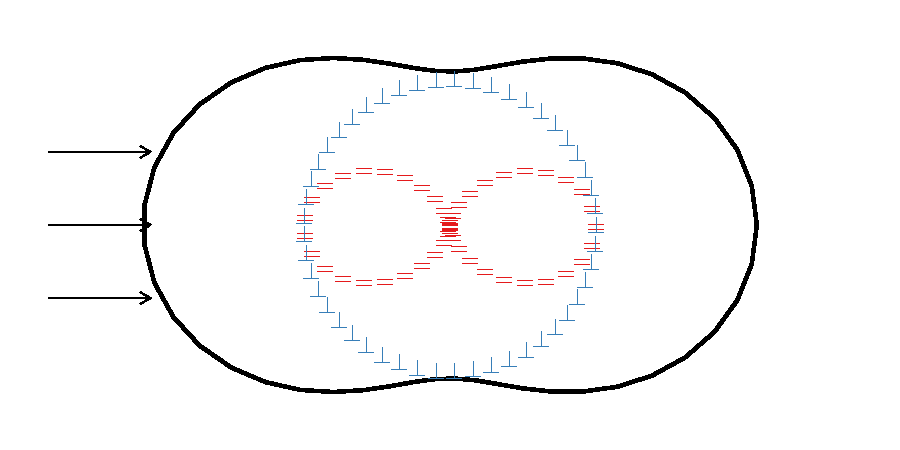
\includegraphics[keepaspectratio, width = 1\linewidth]{images/scat_00.pdf}
    \caption{
        The angular distribution of scattered radiation.
        The blue `$\perp$' symbols denote the intensity of radiation polarized perpendicular to the scattering plane,
        the red `$=$' symbols -- the intensity of radiation polarized parallel to the scattering plane.
        The black solid line shows the sum of the two components.
    }
    \label{fig:simple_scat}
\end{figure}

The simplest case is Thomson scattering on stationary electrons, which is described by a single parameter -- scattering angle $\Theta$.
For a single scattering, the Stokes parameters of the scattered ray $\vctr{S}^\prime$ can be expressed through the Stokes parameters of the incident ray $\vctr{S}$ using the following relationship \citep{Cha60}: 
\begin{equation}
    \vctr{S}^\prime = \frac{f_\mrm{Th}}{2}
    \begin{bmatrix}
        1 + \cos^2\Theta & \cos^2\Theta - 1 & 0 & 0 \\
        \cos^2\Theta - 1 & 1 + \cos^2\Theta & 0 & 0 \\
        0 & 0 & 2\cos\Theta & 0 \\
        0 & 0 & 0 & 2\cos \Theta
    \end{bmatrix}
    \vctr{S},
\end{equation} 
where $f_\mrm{Th}$ is the dilution factor and transformation matrix is the Mueller matrix \citep[$\mtrx{M}_\mrm{Th}$;][]{PolarizedLight2}.
The intensity of the scattered radiation is shown in Fig.~\ref{fig:simple_scat}.
The intensity of the component, polarized perpendicular to the scattering plane ($\vctr{S}_\mrm{inc} = I_0[1, -1, 0, 0]^\mrm{T}$), is independent of the scattering angle $\Theta$.
The radiation polarized parallel to the scattering plane ($\vctr{S}_\mrm{inc} = I_0[1, 1, 0, 0]^\mrm{T}$), is scattered proportional to the $\cos^2\Theta$ \citep{LightScat}.
Thus, if the incident radiation is unpolarized, it can be decomposed into two linearly polarized rays, and the scattered radiation is polarized perpendicular to the scattering plane.
The degree of linear polarization is
\begin{equation}
    P(\Theta) = \frac{I_\perp(\Theta) - I_\parallel(\Theta)}{I_\perp(\Theta) + I_\parallel(\Theta)},
\end{equation}
and reaches maximum of 100\% at $\Theta = \pi/2$. 


A more sophisticated case is Compton scattering -- inelastic scattering involving energy exchange between photon and, for example, electron.
Two scenarios are possible: Compton scattering on slow (thermal) electrons, during which photon loses part of its energy, accelerating charged particle, and inverse Compton scattering (sometimes referred to as \textit{upscattering}) on relativistic electrons, during which photons gain energy from the scattering particle.
While geometrical treatment of Compton effect is similar to that of Thomson, energy exchange should be incorporated into the Compton effect Mueller matrix \citep{PolarizedLight2}:
\begin{equation}
    \vctr{S}^\prime = \frac{f_\mrm{C}}{2}
    \begin{bmatrix}
        \cos^2\Theta + 2\mathcal{B} - 1 & \cos^2\Theta - 1 & 0 & 0 \\
       \cos^2\Theta - 1 & 1 + \cos^2\Theta & 0 & 0 \\
        0 & 0 & 2\cos\Theta & 0 \\
        0 & 0 & 0 & 2\mathcal{B}\cos \Theta
    \end{bmatrix} \vctr{S},
\end{equation}
where $\mathcal{B} = \frac{1}{2}\left(\frac{\nu_\mrm{i}}{\nu_\mrm{s}} + \frac{\nu_\mrm{s}}{\nu_\mrm{i}}\right)$, $\nu_\mrm{i}$ is the incident ray frequency, $\nu_\mrm{s} = \nu_\mrm{i}\left(1 + \frac{h\nu_\mrm{i}}{m_\mrm{e}c^2}(1 - \cos\Theta)\right)^{-1}$ is the scattered ray frequency.
If Mueller matrices of Thomson and Compton scatterings are denoted as $\mtrx{M}_\mrm{Th}(\Theta)$ and $\mtrx{M}_\mrm{C}(\Theta)$, respectively, then $\mtrx{M}_\mrm{C}(\Theta) = \mtrx{M}_\mrm{Th}(\Theta) + \mtrx{M}_\mrm{D}(\Theta)$, where 
\begin{equation}
    \mtrx{M}_\mrm{D}(\Theta) =  2(\mathcal{B} - 1)
    \begin{bmatrix}
        1 & 0 & 0 & 0\\
        0 & 0 & 0 & 0 \\
        0 & 0 & 0 & 0 \\
        0 & 0 & 0 & \cos\Theta
    \end{bmatrix}
\end{equation}
describes additional changes in intensity and circular polarization as a result of energy redistribution associated with the inelastic scattering. 

The Compton scattering in general can be described by Mueller matrix of the following form:
\begin{equation}
    \mtrx{M}_\mrm{C}\left(\nu_i, \nu_s, \Theta\right) = 
    \begin{bmatrix}
        S & S_\mrm{I} & 0 & 0 \\
        S_\mrm{I} & S_\mrm{Q} & 0 & 0 \\
        0 & 0 & S_\mrm{U} & 0 \\
        0 & 0 & 0 & S_\mrm{V} \\
    \end{bmatrix},
\end{equation}
which is obtained by averaging the Compton scattering redistribution matrix over the electron distribution \citep{Nagirner1993}.
The deviation from the Thomson scatterring can be observed on a sample Maxwellian electron distribution.
Unpolarized incident light becomes partially linearly polarized to a degree of $P_\mrm{Th} = (\cos^2\Theta - 1) / (1 + \cos^2\Theta)$ in Thomson regime.
In Compton regime, $P_\mrm{C} = S_\mrm{I} / S$, which is similar to Thomson scattering if the electron temperature is low. 
At high temperatures $P_\mrm{C}$ becomes smaller than $P_\mrm{Th}$ by a factor of few \citep[dependening on the scattering angle $\Theta$ and ratio of $\nu_i/\nu_s$, see ][]{Poutanen1993}.
If the incident radiation is fully linearly polarized, Thomson scattering produces also fully linearly polarized radiation, but may affect the \gls{PA}.
For $q$-polarized incident radiation $I[1, 1, 0, 0]^\mrm{T}$, $P_\mrm{C}^q = (S_\mrm{I} + S_\mrm{Q}) / (S + S_\mrm{I}) \le 1$.
For the case of incident $u$-polarized radiation $I[1, 0, 1, 0]^\mrm{T}$, $P_\mrm{C}^u = \sqrt{S_\mrm{I}^2 + S_\mrm{U}^2} / S \le 1$ \citep[see also][]{Poutanen1993a}.

The degree of linear polarization introduced by Compton scattering is systematically smaller than that by Thomson scattering, and the depolarization effect grows with the electron temperature.
This phenomenon becomes important when low-energy photons are upscattered by hot electrons, which is observed in \glspl{BHXRB} in the hard state \citep{Zdziarski2004a,Poutanen2014a}.


Rayleigh scattering on particles of different sizes plays important role in the atmospheres, including that of the Earth.
This type of scattering is elastic (no energy redistribution between different wavelengths) and occurs when the size of the scattering particle is much smaller than the wavelength of the incident radiation \citep{AbsorbScat}. 
The formal requirement is $2\pi a/\lambda |m(\lambda)| \ll 1$, where $a$ is the size of the particle, $m(\lambda) = n(\lambda) + ik(\lambda)$ is the complex refractive index, real part of which corresponds to the phase speed of the wave in the medium, and imaginary part -- to the extinction \citep{LightScat}.
While \gls{PD} depends on the scattering angle as e.g. in Thomson scattering, the intensity is highly sensitive to the wavelength of the incident radiation \citep{AbsorbScat}:
\begin{equation}
    \vctr{S}^\prime = f_\mrm{R} \frac{1}{\lambda^4}\left|\frac{m(\lambda)^2 - 1}{m(\lambda)^2 + 2}\right|^2\mtrx{M}_\mrm{Th}(\Theta)\vctr{S}.
\end{equation}
Thus, if $m(\lambda)$ varies slowly with $\lambda$, $I_\mrm{scat} \propto \frac{1}{\lambda^4}(1 + \cos^2\Theta) I_\mrm{inc}$, $I_\mrm{scat}$ and $I_\mrm{inc}$ being scattered and incident radiation intensities, respectively. 


\subsection{Polarization by the interstellar medium}
\label{sec:pol_ism}
Much like interstellar absorption, polarization of the \gls{ISM}, which was independently discovered in 1949 by John Hall \citep{Hall1949} and William Hiltner \citep{Hiltner1949}, plays an important role in studying distant objects.
On the line of sight between the target and the observer there may exist a number of scattering clouds, some of them consist of the dust particles.
Dust particles are large and asymmetric, which makes them susceptible to the external ordered magnetic fields.

When a source is observed through a dust cloud, the light is scattered by the dust particles.
The non-sphericity of the particles causes them to have different cross-sections for the orthogonally polarized components of the radiation.
This effectively translates into different absorption coefficients for different components, and, as a result, introduces a difference between the intensities of orthogonally polarized rays.

A cloud of randomly oriented non-spherical dust particles produces no net polarization.
However, the Galactic magnetic field can align some of the silicate grains, creating a preferred orientation within the cloud \citep{Mathis1986, Li1997}, which produces interstellar linear polarization in the direction of the magnetic field lines.


Both the laws of the interstellar extinction and polarization can be established empirically through thorough observations of targets at different galactic coordinates.
The extinction is reasonably well approximated by the model of \citet{Cardelli89} and \citet{ODonnell94}
\begin{equation}
    \frac{A(\lambda)}{A_V} = a(\lambda) + \frac{b(\lambda)}{R_V},
\end{equation}
where $A(\lambda)$ is extinction at wavelength $\lambda$, such that $I_\mrm{obs}(\lambda) = I_\mrm{src}(\lambda) \times 10^{-A(\lambda)/2.5}$, $A_V$ is extinction in $V$-filter, $a(\lambda)$ and $b(\lambda)$ are polynomials of $1/\lambda$, and $R_V = A_V / E(B-V)$ is the ratio of the visual extinction to reddening.
The best-fit value of $R_V$ is $\sim 3.1$ \citep[based on a sample of stars, see][]{ODonnell94}, however it may deviate from the fit value depending on the properties of the \gls{ISM} in a given direction.
The interstellar polarization can be described by the Serkowski law \citep{Serkowski1962, Serkowski1973, Whittet1992}
\begin{equation}
    \label{eq:pol_serkowski}
    \frac{P(\lambda)}{P_\mrm{max}} = \exp\left(-K\left(\lambda_\mrm{max}\right) \ln^2\frac{\lambda_\mrm{max}}{\lambda} \right),
\end{equation}
where $P(\lambda)$ is the observed degree of linear polarization, $P_\mrm{max}$ is the maximum polarization reached at $\lambda_\mrm{max}$.
The \gls{PA} is wavelength-independent.

Dust grains that cause the \gls{IS} polarization also contribute to the \gls{IS} extinction, which results in a tight relationship between the magnitude of \gls{IS} polarization and absorption.
Let $n(a, s)$ be the number density distribution of cylindrical dust grains as a function of grain size $a$ and distance $s$, $C_\parallel\left(a, \lambda\right)$ and $C_\perp\left(a, \lambda\right)$ -- the average extinction cross-sections for radiation, polarized parallel and perpendicular to the grain symmetry axis, respectively.
The \gls{IS} extinction and linear polarization as functions of wavelength $\lambda$ can then be written as follows \citep{LightScat, Li1997,Voshchinnikov2012}:
\begin{align}
    A(\lambda) &= \frac{2.5}{\ln(10)} \displaystyle\int\limits_0^{S}\dd s \int\limits_{a_\mrm{min}}^{a_\mrm{max}} n(a, s) \left(C_\parallel(a, \lambda) + C_\perp(a, \lambda)\right) \dd a , \\
    P(\lambda) &= \int\limits_0^{S}\dd s \int\limits_{a_\mrm{min}}^{a_\mrm{max}} n(a, s) \left(C_\parallel(a, \lambda) - C_\perp(a, \lambda)\right) \dd a ,
\end{align} 
where $S$ is distance to the source, $a_\mrm{min}$ and $a_\mrm{max}$ are the lower and upper size limits of the dust grain distribution.
In the simplest scenario, the ratio of \gls{PD} to the optical depth is determined by the difference in the extinction cross-sections:
\begin{equation}
\frac{P(\lambda)}{\tau(\lambda)} = \left\langle\frac{|C_\parallel(a, \lambda) - C_\perp(a, \lambda)|}{C_\parallel(a, \lambda) + C_\perp(a, \lambda)}\right\rangle_a.
\end{equation}
There exists an empirical limit of the maximum \gls{IS} polarization to the visual extinction ratio, $P_\mrm{max} / A_V \lesssim 3\%~\mrm{mag}^{-1}$, which is equivalent to $P_\mrm{max} \lesssim 9\%~E(B-V)$, assuming $R_V = 3.1$ \citep{Serkowski1975}.


It is worth noting that interstellar extinction is a cumulative quantity -- the more absorbing media are present on the line of sight, the larger the extinction.
However, this is not always the case for the polarization. 
Linear polarization is a pseudo-vector, therefore if, for example, two dust clouds along the line of sight introduce large linear polarization with \glspl{PA} offset by $90^\circ$, the observed emission will show little to no \gls{ISM} polarization, but will be heavily extinct.

A dust cloud can be viewed as a linear polarizer, which is a valid approximation when considering only linear polarization.
Circular polarization requires a more careful treatment and, in general, solution of radiative transfer equations for Stokes parameters \citep{Martin1974}.
The polarization introduced by such cloud can be expressed using the following matrix operator \citep{PolarizedLight2}:
\begin{equation}
    \mtrx{M}\left(A, \delta\right) = \frac{A}{2} 
    \begin{bmatrix}
        1 & \cos 2\delta & 0 & 0 \\
        \cos 2\delta & 1 & 0 & 0 \\
        0 & 0 & \sin 2\delta & 0 \\
        0 & 0 & 0 & \sin 2\delta \\        
    \end{bmatrix},
\end{equation}
where $0 \le A \le 1$ denotes the total absorption coefficient (the fraction of emission that is not absorbed by the cloud) and $\delta$ describes the difference between absorption of light polarized parallel and perpendicular to the magnetic field lines, such that $A_\parallel = A\cos^2 \delta$ and $A_\perp = A\sin^2 \delta$.
Two clouds with magnetic field orientations $\varphi_1$ and $\varphi_2$, located along the line of sight between the observer and the source, are described by the operator
\begin{equation}
    \begin{aligned}
        \mtrx{M}\left(A_1, \delta_1, \varphi_1, A_2, \delta_2, \varphi_2\right) = &\\ 
        \mtrx{M}_\mrm{rot}(-\varphi_2) \mtrx{M}\left(A_2, \delta_2\right) & \mtrx{M}_\mrm{rot}(\varphi_2) 
        \mtrx{M}_\mrm{rot}(-\varphi_1) \mtrx{M}\left(A_1, \delta_1\right)  \mtrx{M}_\mrm{rot}(\varphi_1).
    \end{aligned}
\end{equation}

If the distant source emits unpolarized light $\vctr{S} = [I, 0, 0, 0]^\mrm{T}$, then the first cloud introduces the following linear polarization:
\begin{equation}
    \vctr{S}_1 = \mtrx{M}_\mrm{rot}(-\varphi_1) \mtrx{M}\left(A_1, \delta_1\right)  \mtrx{M}_\mrm{rot}(\varphi_1) \vctr{S} = I\frac{A_1}{2}
    \begin{bmatrix}
        1\\
        \cs{1}{2\delta}\cs{1}{2\varphi}\\
        \cs{1}{2\delta}\sn{1}{2\varphi}\\
        0\\
    \end{bmatrix},
\end{equation}
where $\cs{i}{\alpha} \equiv \cos\alpha_i$ and $\sn{i}{\alpha} \equiv \sin\alpha_i$.
The partially absorbed and polarized light then propagates through the second cloud
\begin{equation}
    \vctr{S}_2 = \mtrx{M}_\mrm{rot}(-\varphi_2) \mtrx{M}\left(A_2, \delta_2\right)  \mtrx{M}_\mrm{rot}(\varphi_2) \vctr{S}_1.
\end{equation}
$\vctr{S}_2$ is the Stokes vector of the observed light.
It can be expressed in terms of the intensity $I$ of the source unpolarized radiation and properties of the dust clouds:
\begin{multline}
    \vctr{S}_2 = I\frac{A_2}{2}\frac{A_1}{2} \times \\
    \times 
    \begin{bmatrix}
        1 + \cs{2}{2\delta}\cs{1}{2\delta}\cos\left(2\varphi_2 - 2\varphi_1\right) \\
%
        \cs{2}{2\delta}\cs{2}{2\varphi} + \cs{1}{2\delta}\left[\left(\left(\cs{2}{2\varphi}\right)^2 + \sn{2}{2\delta}\left(\sn{2}{2\varphi}\right)^2\right)\cs{1}{2\varphi} + \frac{1}{2}\left(1 - \sn{2}{2\delta}\right)\sn{2}{4\varphi}\sn{1}{2\varphi}\right]\\
%
        \cs{2}{2\delta}\sn{2}{2\varphi} + \cs{1}{2\delta}\left[\frac{1}{2}\left(1 - \sn{2}{2\delta}\right)\sn{2}{4\varphi}\cs{1}{2\varphi} + \left(\left(\sn{2}{2\varphi}\right)^2 + \sn{2}{2\delta}\left(\cs{2}{2\varphi}\right)^2 \right)\sn{1}{2\varphi}\right] \\
%
        0
    \end{bmatrix}.
\end{multline}
The total intensity decreases by at least a factor $\frac{1}{2}A_2A_1$.
The maximum intensity is achieved if dust grains in both clouds are oriented in the same direction ($\left|\varphi_1 - \varphi_2\right| \approx 0$), and clouds fully polarize incoming light ($\cs{1}{\delta} = \cs{2}{\delta} = 1$).
In this case, the observed light is also fully linearly polarized:
\begin{equation}
    \vctr{S}^\prime = \frac{1}{2}A_2A_1I \left[1, \cos2\varphi, \sin2\varphi, 0\right]^\mrm{T}.
\end{equation}

If the magnetic field lines in the clouds are almost orthogonal to each other, i.e. $\left|\varphi_1 - \varphi_2\right| \approx \pi/2$, then the observed flux decreases substantially.
In the simplest case of $\varphi_1 = 0$ and $\varphi_2 = \pi/ 2$, the observed Stokes vector is 
\begin{equation}
\vctr{S}^\prime = \frac{1}{4}A_2A_1I \left[1 - \cs{2}{2\delta}\cs{1}{2\delta}, \cs{1}{2\delta} - \cs{2}{2\delta}, 0, 0\right]^\mrm{T}.
\end{equation}
Here $0 \le \cs{i}{2\delta} \le 1$, which are equivalent to the linear \gls{PD} produced by each cloud.
The observed \gls{PD}, $p = \left|\cs{1}{2\delta} - \cs{2}{2\delta}\right|/\left(1 - \cs{2}{2\delta}\cs{1}{2\delta}\right)$, can be small, and polarization angle can be either $0$ or $\pi / 2$.

A similar approach can be used to determine the effect of a dust cloud on the partially linearly polarized source radiation.
Let $\vctr{S} = I[1, p\cos2\alpha, p\sin2\alpha, 0]^\mrm{T}$ be the Stokes vector of the emitted radiation, where $I$ is the total intensity, $p$ is the \gls{PD}, $\alpha$ is the \gls{PA}.
Let the dust cloud on the line of sight be described with parameters $A$, $\varphi$, and $\delta$.
Assuming that $p \ll 1$ (source polarization degree is small) and $\cos2\delta \ll 1$ (the dust cloud introduces small linear polarization), the observed Stokes vector of the light that passed through singular dust cloud is
\begin{equation}
    \label{eq:pol_small_p_approx}
    \vctr{S}^\prime \approx \frac{1}{2} A I 
    \begin{bmatrix}
        1 + p p_\mrm{ism}\cos(2\alpha - 2\varphi) \\
        p_\mrm{ism}\cos2\varphi + p\cos2\alpha \\
        p_\mrm{ism}\sin2\varphi + p\sin2\alpha \\
        0
    \end{bmatrix},
\end{equation}
where $p_\mrm{ism} \equiv \cos2\delta$ is the \gls{PD} of the \gls{ISM}.
The observed degree of polarization is then 
\begin{equation}
    p^\prime \approx \sqrt{p_\mrm{ism}^2 + p ^ 2 + 2pp_\mrm{ism}\cos\left(2\varphi - 2\alpha\right)},
\end{equation}
assuming $pp_\mrm{ism} \lll 1$.
$p^\prime$ lies within the $[|p - p_\mrm{ism}|;~p + p_\mrm{ism}]$ interval.
The observed polarization angle $\theta$ can be obtained from the following relationship:
\begin{equation}
    \tan 2\theta \approx \tan 2\alpha \frac{1 + \frac{p_\mrm{ism}}{p} \frac{\sin2\varphi}{\sin 2\alpha}}{1 + \frac{p_\mrm{ism}}{p}\frac{\cos2\varphi}{\cos2\alpha}}.
\end{equation}
As a result, the \gls{ISM} can affect polarization of the radiation, converting unpolarized light from the source into (partially) linearly polarized, and changing observed polarization angle and degree.
This effect can cause a depolarization of the source light, especially when \gls{PD} of the emitted light is comparable to the \gls{PD}, introduced by the \gls{ISM}.

Eq.~\ref{eq:pol_small_p_approx} can be used to illustrate another important property of the \gls{ISM} polarization:
\begin{equation}
    \vctr{S}^\prime \approx \frac{1}{2} A I \left(
        \begin{bmatrix}
            1 - p - p_\mrm{ism} \\ 0 \\ 0 \\ 0 \\
        \end{bmatrix}  + p_\mrm{ism} 
        \begin{bmatrix}
            1 \\ \cos2\varphi \\ \sin2\varphi \\ 0 \\
        \end{bmatrix} + p
        \begin{bmatrix}
            1 \\ \cos2\alpha \\ \sin2\alpha \\ 0 \\
        \end{bmatrix}
    \right).
\end{equation}
The observed emission can be decomposed into unpolarized, \gls{ISM} and intrinsic fully linearly polarized components.
If \gls{ISM} polarization is determined independently (e.g., by studying field stars), it can be subtracted form the observed polarization of the source, allowing to measure the intrinsic polarization.

\begin{figure}
    \centering
    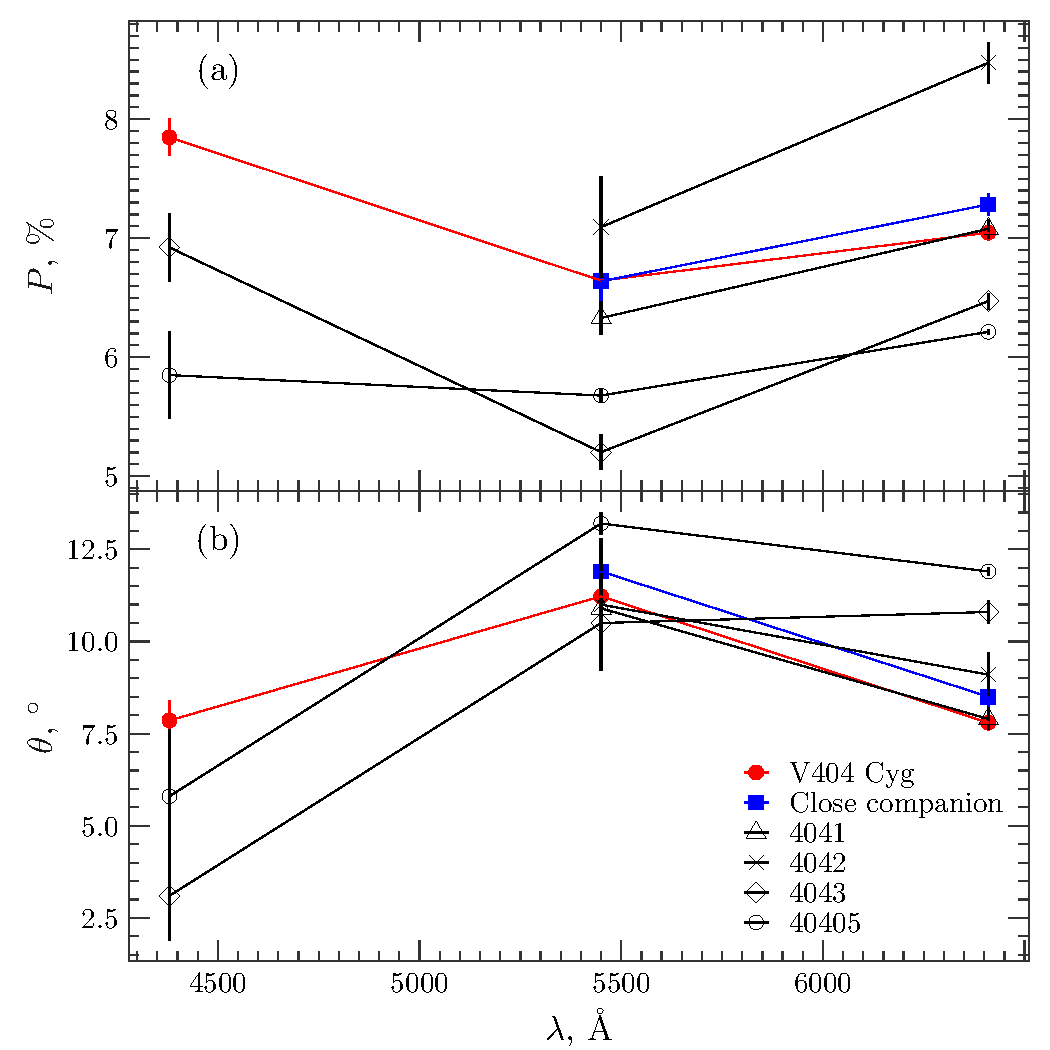
\includegraphics[keepaspectratio, width = 0.95\linewidth]{images/field__7.pdf}
    \caption{
        Wavelength dependence of polarization degree (top panel) and angle (bottom panel) of V404~Cyg in quiescence after 2015 outburst, its visually close companion, and field stars.
        Errors are 1$\sigma$.
        From \paperII.
    }
    \label{fig:pol_v404_field}
\end{figure}
Multiple clouds on the line of sight can produce a complex dependence of \gls{PD} on wavelength.
Polarization, produced by each cloud, can be described using the Serkowski law (Eq.~\ref{eq:pol_serkowski}).
If $\lambda_\mrm{max}$ and \glspl{PA} are different, the observed \gls{ISM} polarization deviates from the Serkowski law.
Such effect has been observed in \gls{BHXRB} \VCYG\ and field stars around it (see Fig.~\ref{fig:pol_v404_field}).
The stars exhibit large (up to 8.5\% in $R$) wavelength-dependent \gls{ISM} polarization with a local minimum in $V$ filter and variable \gls{PA}. 
Such polarization spectra cannot be described by a single Serkowski curve, which suggests that multiple polarizing dust clouds contribute to the observed polarization.
These clouds can be also responsible for high \gls{IS} absorption in the direction of \VCYG\ ($A_V$ up to 4.4, \citealt{Shahbaz2003}).

Multiple dust clouds can produce circular polarization of the unpolarized incident radiation.
The mechanism can be understood under the assumption that asymmetric dust particles of the two sample clouds are oriented at different position angles with respect to some direction on the sky ($\varphi_1$ and $\varphi_2$).
If both clouds are optically thin, such that $\tau_{1,2}^{\perp, \parallel} \ll 1$ are optical depths for the radiation polarized perpendicular and parallel to the plane containing wave vector $\vctr{k}$ and dust particle orientation vector, then the circular polarization degree of the incident light that sequentially passed through these two clouds can be expressed as follows \citep{PolarizationInCosmicMedium}:
\begin{equation}
    P_\mrm{circ} = \frac{1}{4}\left(\tau_1^\parallel - \tau_1^\perp\right)\left(\tau_2^\parallel - \tau_2^\perp\right) \sin\left(2\left(\varphi_1 - \varphi_2\right)\right)\frac{\mrm{Re}\left(m_2^\parallel - m_2^\perp\right)}{\mrm{Im}\left(m_2^\parallel - m_2^\perp\right)},
\end{equation}
where $m_2^{\perp,\parallel}$ are refractive indices of the second cloud for orthogonally polarized waves.
However, the degree of circular polarization is proportional to the product of the average difference of the optical depths of two clouds, which makes $P_\mrm{circ}$ a small quantity compared to the degree of linear polarization in the case of the optically thin media.

This effect is prominent when the incident light is linearly polarized by, e.g., a more distant cloud. 
Two optically thin clouds  with nearly orthogonal orientation of the dust particles partly transform linearly polarized light into circular.
Such circular polarization has typical value of $\sim10^{-2}\%$ and is detected for several high-linearly polarized stars (see, e.g., \citealt{Martin1976}).

\subsection{Depolarizing effects}

A combination of multiple polarizing effects can actually lead to the net depolarization of emission.
Such is the case of Faraday rotation, which may introduce circular polarization or rotate the polarization plane, affecting the observed \gls{PA}.
If different emitting regions suffer from unequal Faraday rotation, the net observed polarization may be significantly reduced.

A careful treatment of radiative transfer equation for Stokes parameters gives the following relationship between emitted $\vctr{S}_0$ and transferred $\vctr{S}$ Stokes vectors:
\begin{equation}
    \label{eq:radiative_transport_stokes}
    \vctr{S} = 
    \left(\mtrx{I}_4 - 
    \begin{bmatrix}
        \tau & \tau_Q & \tau_U & \tau_V \\
        \tau_Q & \tau & -\psi_V & \psi_U \\
        \tau_U & \psi_V & \tau & -\psi_Q \\
        \tau_V & -\psi_U & \psi_Q & \tau
    \end{bmatrix}\right)
    \vctr{S}_0,
\end{equation}
where $\mtrx{I}_4 = \mrm{diag}(1, 1, 1, 1)$ is identity matrix, $\tau$ is the Thomson optical depth, $\tau_{\{Q, U, V\}}$ are determined by the dichroism of the medium in respect to linear and circular polarization, $\psi_{\{Q, U, V\}}$ are phase shifts, which describe the birefringence of the medium \citep{PolarizationInCosmicMedium}.
In case of Faraday rotation, $\tau_V$ and $\psi_V$ are non-zero.
As a result of Faraday effect, unpolarized emitted radiation $\vctr{S}_0 = I[1, 0, 0, 0]^\mrm{T}$ gains circular polarization $\vctr{S} = I[1-\tau, 0, 0, -\tau_V]^\mrm{T}$, while linearly polarized source radiation $\vctr{S}_0 = I[1, q, u, 0]^\mrm{T}$ experiences a rotation of its polarization angle:
\begin{equation}
    \vctr{S} = 
    I
    \begin{bmatrix}
        1 - \tau \\
        (1 - \tau) q + \psi_V u \\
        (1 - \tau) u - \psi_V q \\
        - \tau_V 
    \end{bmatrix}.
\end{equation}
Taking into account that $q = p_0\cos 2\theta_0$ and $u = p_0\sin 2\theta_0$, $p = p_0 \sqrt{(1 - \tau) ^2 + \psi_V^2} / (1 - \tau)$, and $\theta = \theta_0 - \delta$, where $\delta = 1/2\arctan \left(\psi_V / (1 - \tau)\right)$, assuming $\tau_V$ is negligible.
For relatively small $\psi_V$ (and $\tau_V \ll |\psi_V|$), $p \approx p_0$, $\theta \approx \theta_0 - 0.5\psi_V / (1 - \tau)$.
Although obtained in approximation, the equation for $\theta$ is valid for arbitrary phase shifts $\psi_V$ \citep{PolarizationInCosmicMedium}.

The depolarizing effect of large Faraday rotation angle can be observed in the following example.
If the source is a combination of emitting regions, each producing linearly polarized emission $I[1, p_0\cos2\theta, p_0\sin2\theta, 0]^\mrm{T}$, but affected by Faraday rotation of different magnitude ($\theta = \theta_0 + \epsilon$, $\epsilon$ is distributed as $f(\epsilon)$), then the average polarization is 
\begin{align}
    \langle\vctr{S}\rangle_\epsilon & = 
    I\begin{bmatrix}
     1 \\
     p_0 \cos2\theta_0\langle\cos2\epsilon\rangle - p_0 \sin2\theta_0\langle\sin2\epsilon\rangle \\   
     p_0 \sin2\theta_0\langle\cos2\epsilon\rangle + p_0\ cos2\theta_0\langle\sin2\epsilon\rangle \\
     0 
    \end{bmatrix}, \\
    \langle\cos2\epsilon\rangle &= \frac{\int\limits_{\epsilon_1}^{\epsilon_2} \cos2\epsilon f(\epsilon) \dd \epsilon}{ \int\limits_{\epsilon_1}^{\epsilon_2}  f(\epsilon) \dd \epsilon}, \\
    \langle\sin2\epsilon\rangle &= \frac{\int\limits_{\epsilon_1}^{\epsilon_2} \sin2\epsilon f(\epsilon) \dd \epsilon}{ \int\limits_{\epsilon_1}^{\epsilon_2}  f(\epsilon) \dd \epsilon}.
\end{align}
The average $p$ scales as $p_0 \sqrt{\langle\cos2\epsilon\rangle^2 + \langle\sin2\epsilon\rangle^2}$.
In the limiting case of $f(\epsilon) = \delta(\epsilon - \epsilon_0)$, $p = p_0$ and no depolarization is observed.
A uniform distribution of $\epsilon$ ($f(\epsilon) = 1$) gives $p = p_0\left|\frac{\sin (\epsilon_2 - \epsilon_1)}{\epsilon_2 - \epsilon_1}\right|$, which decreases proportionally to the magnitude of Faraday rotation, which determines the difference $|\epsilon_2 - \epsilon_1|$.

This effect plays an important role in the hot accretion flow scenario, where
\begin{equation}
|\phi_V| \approx 6.4 \times 10^4 \tau \frac{B_\parallel}{10^6~\mrm{G}} \left(\frac{\nu}{10^{-15}~\mrm{Hz}}\right)^{-2}.
\end{equation}
Here $B_\parallel$ is the component of the magnetic field, parallel to the line of sight \citep[see discussions in ][]{Veledina2013,Poutanen2014a}.
In the \gls{ONIR} frequency range with typical magnetic field of $10^6~\mrm{G}$, the magnitude of $\phi_V$ reaches $10^5$, completely destroying linear polarization.
Thus, in \glspl{LMXB}, large \gls{ONIR} linear polarization of the non-thermal component can be a sign of jet emission, while no linear polarization is a signature of hot accretion flow (as observed in \MAXI, see \paperIII).
